\documentclass[tikz, border=5pt]{standalone}
\usepackage{lmodern}
\usepackage[T1]{fontenc}
\usepackage{tikz}
\usetikzlibrary{shapes.misc, fit, positioning, shapes, arrows, shapes.misc}

\begin{document}
	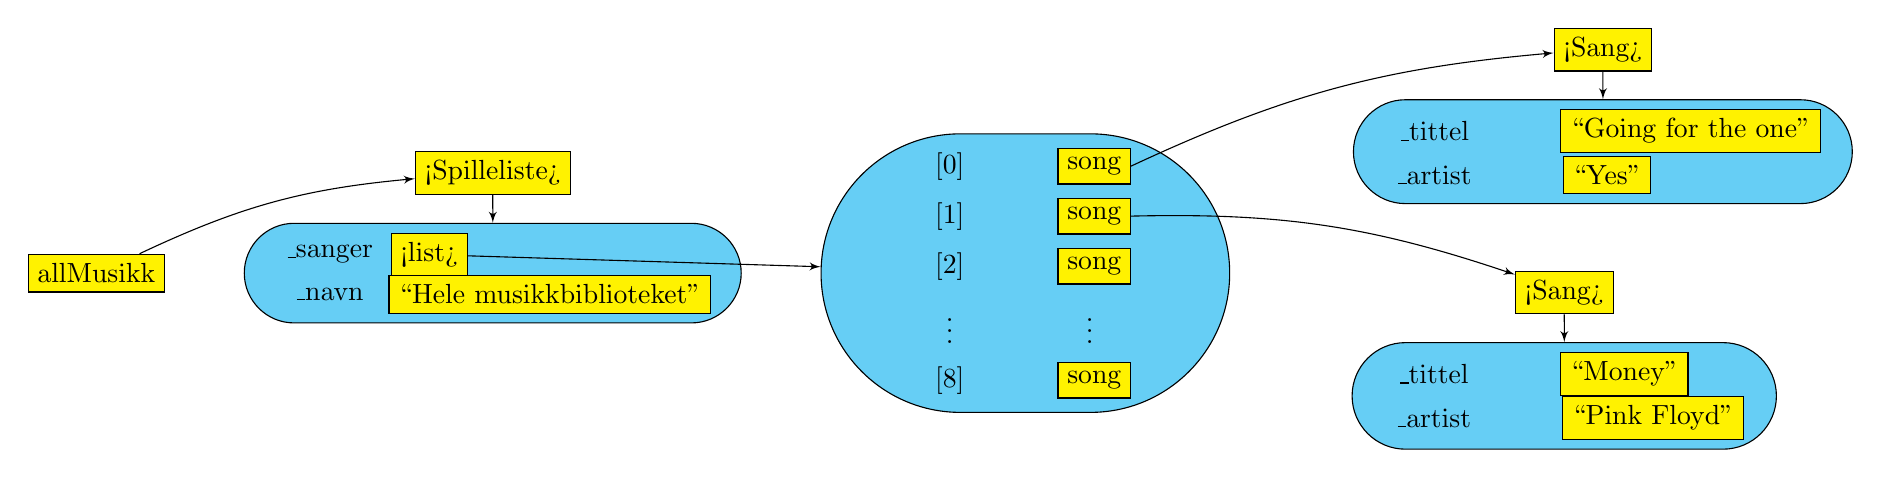
\begin{tikzpicture}
		\node (init) [rectangle, draw, fill=yellow] {allMusikk};
		\node (allmusikk) [matrix, draw, right=of init, rounded rectangle, fill=cyan!60,label={[name=amlabel, rectangle, draw, yshift=10pt, fill=yellow]:<Spilleliste>}] {
			\node (amsanger) {\_sanger};
			\node (amsangervar) [right=2pt of amsanger, rectangle, draw, fill=yellow] {<list>};
			\node (amnavn) [below=2pt of amsanger] {\_navn};
			\node (amnavnvar) [right=5pt of amnavn, rectangle, draw, fill=yellow] {``Hele musikkbiblioteket''}; \\
		};
		\path[draw, -latex'] (init) to[bend left=10] (amlabel);
		\path[draw, -latex'] (amlabel) -> (allmusikk);
		\node (sangliste) [matrix, right=of allmusikk, draw, rounded rectangle, fill=cyan!60] {
			\node (zero) {[0]};
			\node (zerovar) [draw, right=of zero, rectangle, fill=yellow] {song};
			\node (one) [below=1 pt of zero] {[1]};
			\node (onevar) [draw, right=of one, rectangle, fill=yellow] {song};
			\node (two) [below=1 pt of one] {[2]};
			\node (twovar) [draw, right=of two, rectangle, fill=yellow] {song};
			\node (dots) [below=1 pt of two] {\vdots};
			\node (dotsvar) [right=of dots] {\vdots};
			\node (eight) [below=1 pt of dots] {[8]};
			\node (eightvar) [draw, right=of eight, rectangle, fill=yellow] {song};\\
		};
		\path[draw, -latex'] (amsangervar) -> (sangliste);

		\node (firstsong) [matrix, above right=-9mm and 4cm of sangliste, draw, rounded rectangle,label={[name=fslabel, rectangle, draw, yshift=10pt, fill=yellow]:<Sang>}, fill=cyan!60] {
			\node (fstittel) {\_tittel};
			\node (fstittelvar) [right=of fstittel, rectangle, draw, fill=yellow] {``Going for the one''};
			\node (fsartist) [below=2pt of fstittel] {\_artist};
			\node (fsartistvar) [right=of fsartist, rectangle, draw, fill=yellow] {``Yes''};\\
		};
		\node (secondsong) [matrix, below right=-9mm and 4cm of sangliste, draw, rounded rectangle,label={[name=sslabel, rectangle, draw, yshift=10pt, fill=yellow]:<Sang>}, fill=cyan!60] {
			\node (sstittel) {\_tittel};
			\node (sstittelvar) [right=of sstittel, rectangle, draw, fill=yellow, anchor=west] {``Money''};
			\node (ssartist) [below=2pt of sstittel] {\_artist};
			\node (ssartistvar) [right=of ssartist, rectangle, draw, fill=yellow, anchor=west] {``Pink Floyd''};\\
		};
		\path[draw, -latex'] (zerovar.east) to[bend left=10] (fslabel);
		\path[draw, -latex'] (onevar.east) to[bend left=10] (sslabel);
		\path[draw, -latex'] (fslabel) -> (firstsong);
		\path[draw, -latex'] (sslabel) -> (secondsong);
	\end{tikzpicture}
\end{document}
